\label{cap:estado_arte}

\section{Origen y evolución de los robots hexápodos}

El desarrollo de sistemas de locomoción mediante extremidades articuladas ha estado ligado a la robótica bioinspirada, tomando como referencia la morfología y los patrones de movimiento de animales e insectos. Desde el punto de vista de la estabilidad, uno de los trabajos fundacionales fue el de McGhee y Frank \cite{McGhee1968}, quienes estudiaron las secuencias de marcha posibles en robots cuadrúpedos y demostraron que solo un subconjunto reducido garantizaba estabilidad estática. En particular, identificaron seis marchas con al menos tres apoyos, de las cuales solo tres eran estáticamente estables, y solo una maximizaba el margen, coincidiendo con patrones observados en cuadrúpedos en la naturaleza.

Estos principios matemáticos sentaron el estándar para el análisis de cualquier plataforma multípeda. En el caso de los hexápodos, esta teoría explica por qué presentan ventajas en terrenos irregulares: su redundancia mecánica les permite mantener polígonos de soporte mucho más amplios y seguros, como el clásico apoyo en trípode, superando las limitaciones que enfrentan los sistemas de cuatro patas. En esta misma línea, y motivados por la alta eficiencia biomecánica producto de la evolución, numerosos estudios se han dedicado a caracterizar los patrones de locomoción de los artrópodos. Estas investigaciones han revelado que la naturaleza no emplea un único patrón, sino que los insectos se adaptan dinámicamente en función de la velocidad de avance y las características del terreno. Para lograrlo, el sistema nervioso del insecto modula la marcha y el desfase temporal entre el movimiento de sus extremidades, un parámetro conocido como retraso metacronal, tal y como se ilustra en la Figura~\ref{fig:retraso_metacronal_insectos}: la fila superior muestra la alternancia entre los dos trípodes de apoyo, \{I2, D1, D3\} y \{I1, D2, I3\}, y la fila inferior representa, con barras de apoyo y de vuelo, la duración de ese desfase en cada periodo de marcha.

\begin{figure}[htbp]
    \centering
    \captionsetup{justification=centering}
    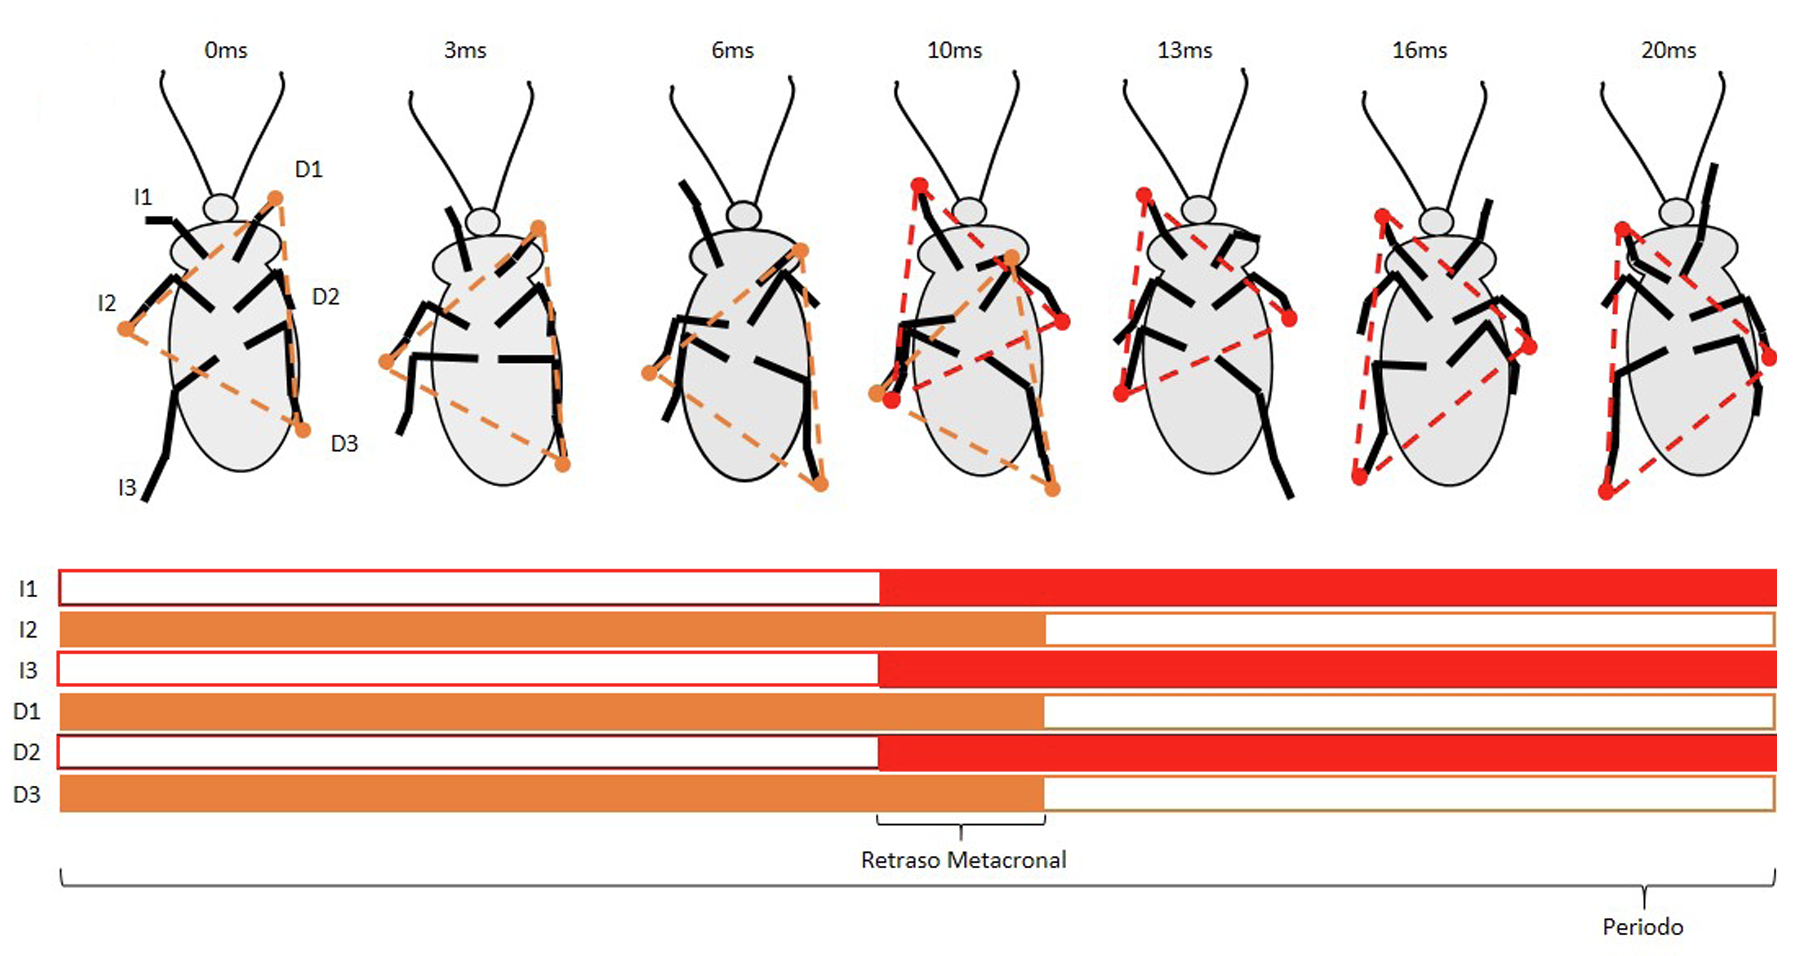
\includegraphics[width=0.60\textwidth]{img/insecto_metacronal.png}
    \caption[Caracterización del patrón en insectos con marcha trípode]{Caracterización del patrón en insectos con marcha trípode\\[-2pt]{\footnotesize Fuente: Fernández-Villalobos (2019) \cite{fernandez2019neurobiologia}.}}
    \label{fig:retraso_metacronal_insectos}
\end{figure}

% --- PRIMERA FIGURA: ODEX I (Derecha) ---
\begin{wrapfigure}[12]{r}{0.35\textwidth}
    \centering
    \captionsetup{justification=centering}
    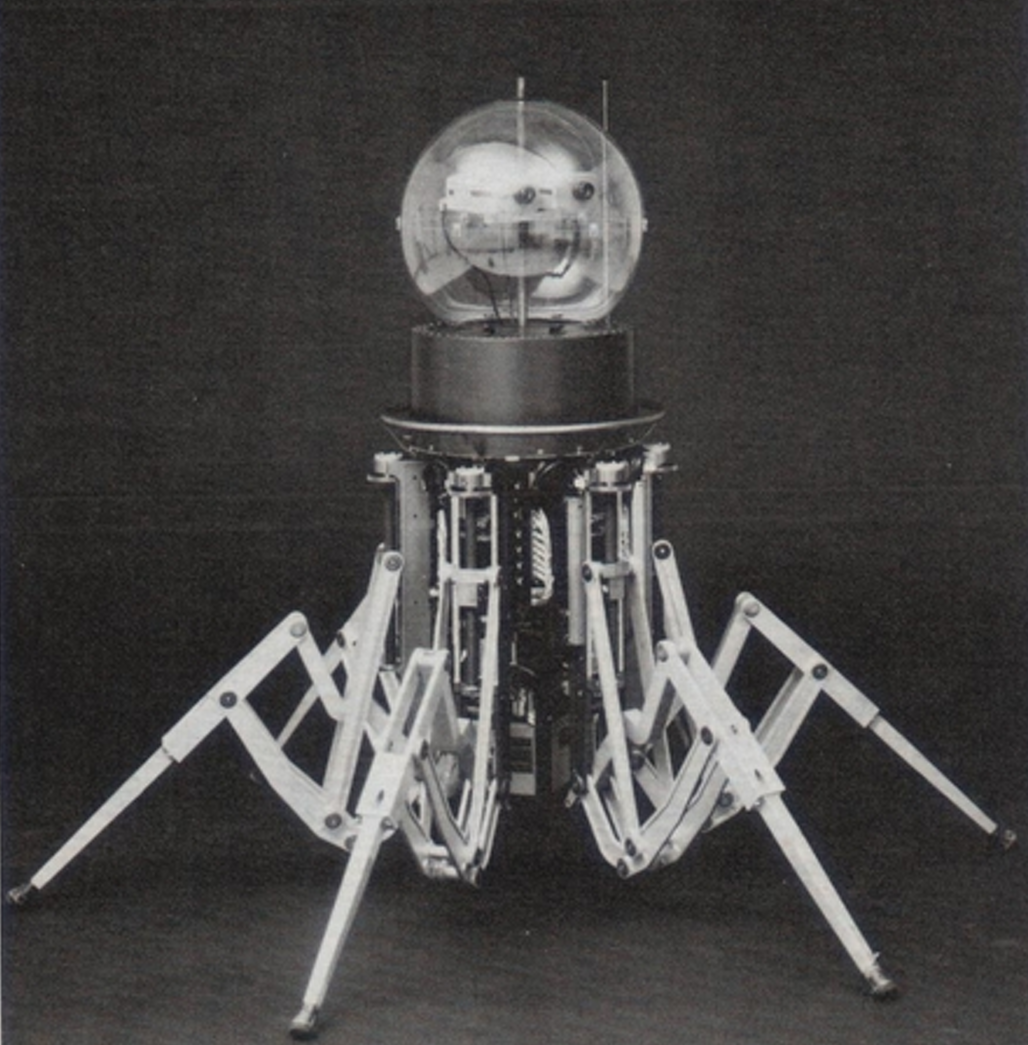
\includegraphics[width=0.30\textwidth]{img/ODEX1.png}
    \caption[Robot ODEX I]{Robot ODEX I\\[-2pt]{\footnotesize Fuente: Russell (1983) \cite{russell1983odex}.}}
    \label{fig:odex1}
    \vspace{-25pt}
\end{wrapfigure}

La traslación de estos principios de locomoción a plataformas electromecánicas supuso un desafío tecnológico. Durante la década de 1980, el desarrollo de robots multípedos experimentó avances fundamentales. Uno de los hitos fue el robot Odex I (ver Figura~\ref{fig:odex1}), presentado en 1983 \cite{russell1983odex}. Este sistema demostró empíricamente la superioridad de los mecanismos articulados de seis patas frente a los vehículos tradicionales de orugas o ruedas, especialmente en la superación de obstáculos geométricos complejos y la navegación en entornos no estructurados. No obstante, su viabilidad estaba restringida por una estructura física sumamente pesada.


% --- SEGUNDA FIGURA: ASV (Izquierda) ---
\begin{wrapfigure}[14]{l}{0.45\textwidth}
    \centering
    \vspace{-15pt}
    \captionsetup{justification=centering}
    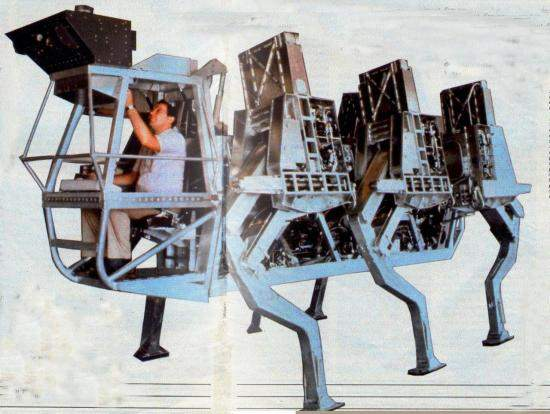
\includegraphics[width=0.45\textwidth]{img/OSU-ASV-1.jpg}
    \caption[Adaptive Suspension Vehicle (ASV)]{Adaptive Suspension Vehicle (ASV)\\[-2pt]{\footnotesize Fuente: Siciliano y Khatib (2016) \cite{siciliano2016springer}.}}
    \label{fig:asv}
    \vspace{-15pt}
\end{wrapfigure}

Poco después, la aplicación a gran escala de las teorías de estabilidad estática se materializó con el \textit{Adaptive Suspension Vehicle} (ASV) en 1986 (ver Figura~\ref{fig:asv}). Resulta especialmente destacable que este proyecto estuviera coliderado por Robert McGhee, aplicando a una plataforma real los modelos matemáticos de locomoción formulados dos décadas atrás \cite{siciliano2016springer,waldron1986asv}. Un sistema de tres toneladas y más de cinco metros de longitud, impulsado por motores de combustión y actuadores hidráulicos, que demostró la viabilidad de la marcha en trípode en un vehículo de escala humana, dependiente de sistemas de computación voluminosos.

% --- TERCERA FIGURA: GENGHIS (Derecha) ---
\begin{wrapfigure}[14]{r}{0.5\textwidth}
    \centering
    \captionsetup{justification=centering}
    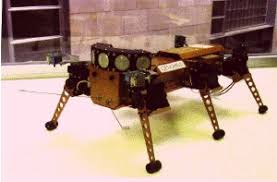
\includegraphics[width=0.5\textwidth]{img/genghis.jpg}
    \caption[Robot Genghis]{Robot \textit{Genghis}\\[-2pt]{\footnotesize Fuente: Brooks (1989) \cite{brooks1989robot}.}}
    \label{fig:genghis}
    \vspace{-20pt}
\end{wrapfigure}

A diferencia de los enfoques convencionales de la época, el MIT introdujo una aproximación alternativa con el robot \textit{Genghis} (ver Figura~\ref{fig:genghis}), que demostró que era posible lograr una locomoción robusta y adaptativa mediante una red de reglas reactivas simples y descentralizadas \cite{brooks1989robot}. En este modelo, cada extremidad operaba a partir de sensores básicos y reflejos locales, de forma análoga al procesamiento neuronal distribuido observado en los insectos. Así, cada pata podía interpretarse como una máquina de estados finitos local, capaz de coordinarse con las demás mediante eventos asíncronos.

A pesar de estos avances, el desarrollo de hexápodos seguía fuertemente condicionado por las restricciones del hardware disponible. Muchas de las primeras plataformas dependían de sistemas hidráulicos o neumáticos, lo que obligaba a operar conectadas a fuentes de alimentación o a incorporar pesados motores de combustión. Estas limitaciones reducían de forma significativa su autonomía, agilidad y viabilidad fuera de entornos experimentales. 


\section{Plataformas hexápodo en la investigación actual}
\label{sec:ea_plataformas}

El desarrollo de plataformas hexápodo en las últimas décadas ha trascendido los altos presupuestos de los años ochenta para consolidarse en un ecosistema accesible. La aparición de las impresoras 3D y el abaratamiento de la electrónica han revolucionado el DIY (Do It Yourself). Además, la resolución continua de los cálculos cinemáticos ya no constituye el principal impedimento, ya que los microcontroladores actuales pueden realizar esta tarea con solvencia. El reto radica en disponer de capacidad computacional suficiente para integrar sistemas de navegación autónoma.

\begin{wrapfigure}[13]{l}{0.38\textwidth}
    \centering
    \vspace{-0.8em}
    \captionsetup{justification=centering}
    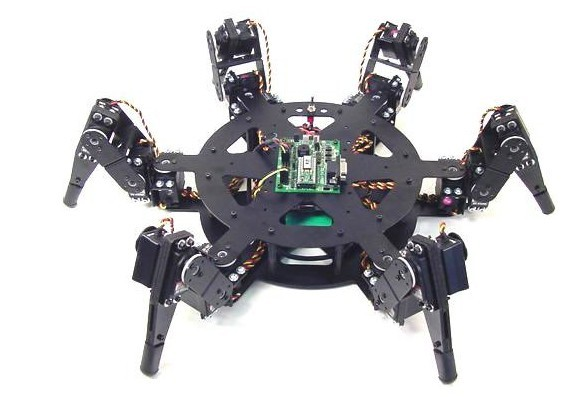
\includegraphics[width=0.38\textwidth]{img/lynxmotion.jpg}
    \caption[Plataforma educativa Lynxmotion]{Lynxmotion\\[-2pt]{\footnotesize Fuente: Lynxmotion \cite{lynxmotion_ses}.}}
    \label{fig:lynxmotion}
    \vspace{-20pt}
\end{wrapfigure}


Dentro del ámbito educativo destacan plataformas basadas en chasis acrílico, o impresión 3D, como los modelos ofrecidos por Freenove \cite{freenove_hexapod} o Lynxmotion \cite{lynxmotion_ses} (ver Figura~\ref{fig:lynxmotion}), que emplean servomotores. Estas soluciones son accesibles, sencillas de montar y adecuadas para introducir conceptos de locomoción multípeda. Sin embargo, no comunican información sensorial al controlador principal y carecen de la telemetría necesaria para implementar estrategias de control reactivo o diagnóstico avanzado. Para superar estas limitaciones, las plataformas orientadas a investigación suelen adoptar actuadores digitales y una arquitectura electrónica más rica. 

\begin{wrapfigure}[11]{r}{0.48\textwidth}
    \centering
    \captionsetup{justification=centering}
    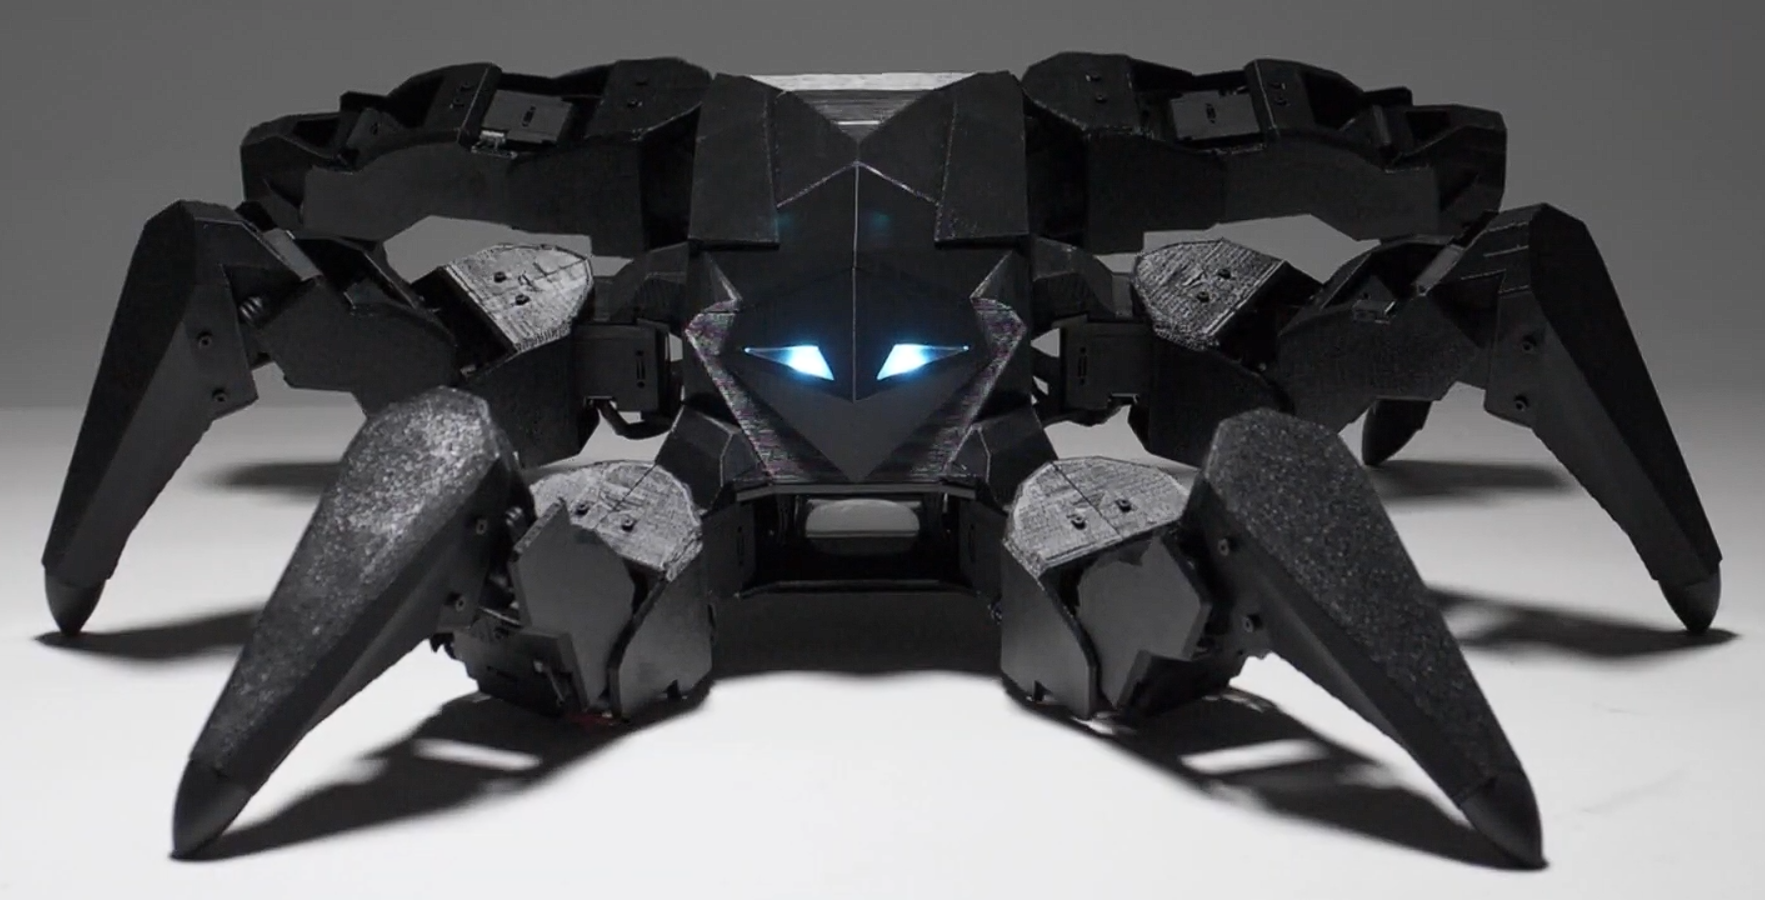
\includegraphics[width=0.45\textwidth]{img/mark4.png}
    \caption[PhantomX Hexapod Mark IV]{PhantomX Mark IV\\[-2pt]{\footnotesize Fuente: Trossen Robotics \cite{phantomx_mk4}.}}
    \label{fig:mark4}
    \vspace{-25pt}
\end{wrapfigure}

En este ámbito destaca la familia \textit{PhantomX} de Trossen Robotics, que ha evolucionado hasta el \textit{PhantomX Mark IV} (ver Figura~\ref{fig:mark4}), una actualización orientada a investigación avanzada. Esta versión incorpora una Raspberry Pi para facilitar la integración con ROS 2 y actualiza los actuadores a nuevas generaciones de la serie X de DYNAMIXEL \cite{robotis_xseries}. Aun así, numerosos trabajos continúan empleando el \textit{PhantomX Mark III}, mencionado en la introducción, por su disponibilidad y por la amplia base de software y documentación.


\begin{wrapfigure}[11]{l}{0.43\textwidth}
    \centering
    \vspace{-0.8em}
    \captionsetup{justification=centering}
    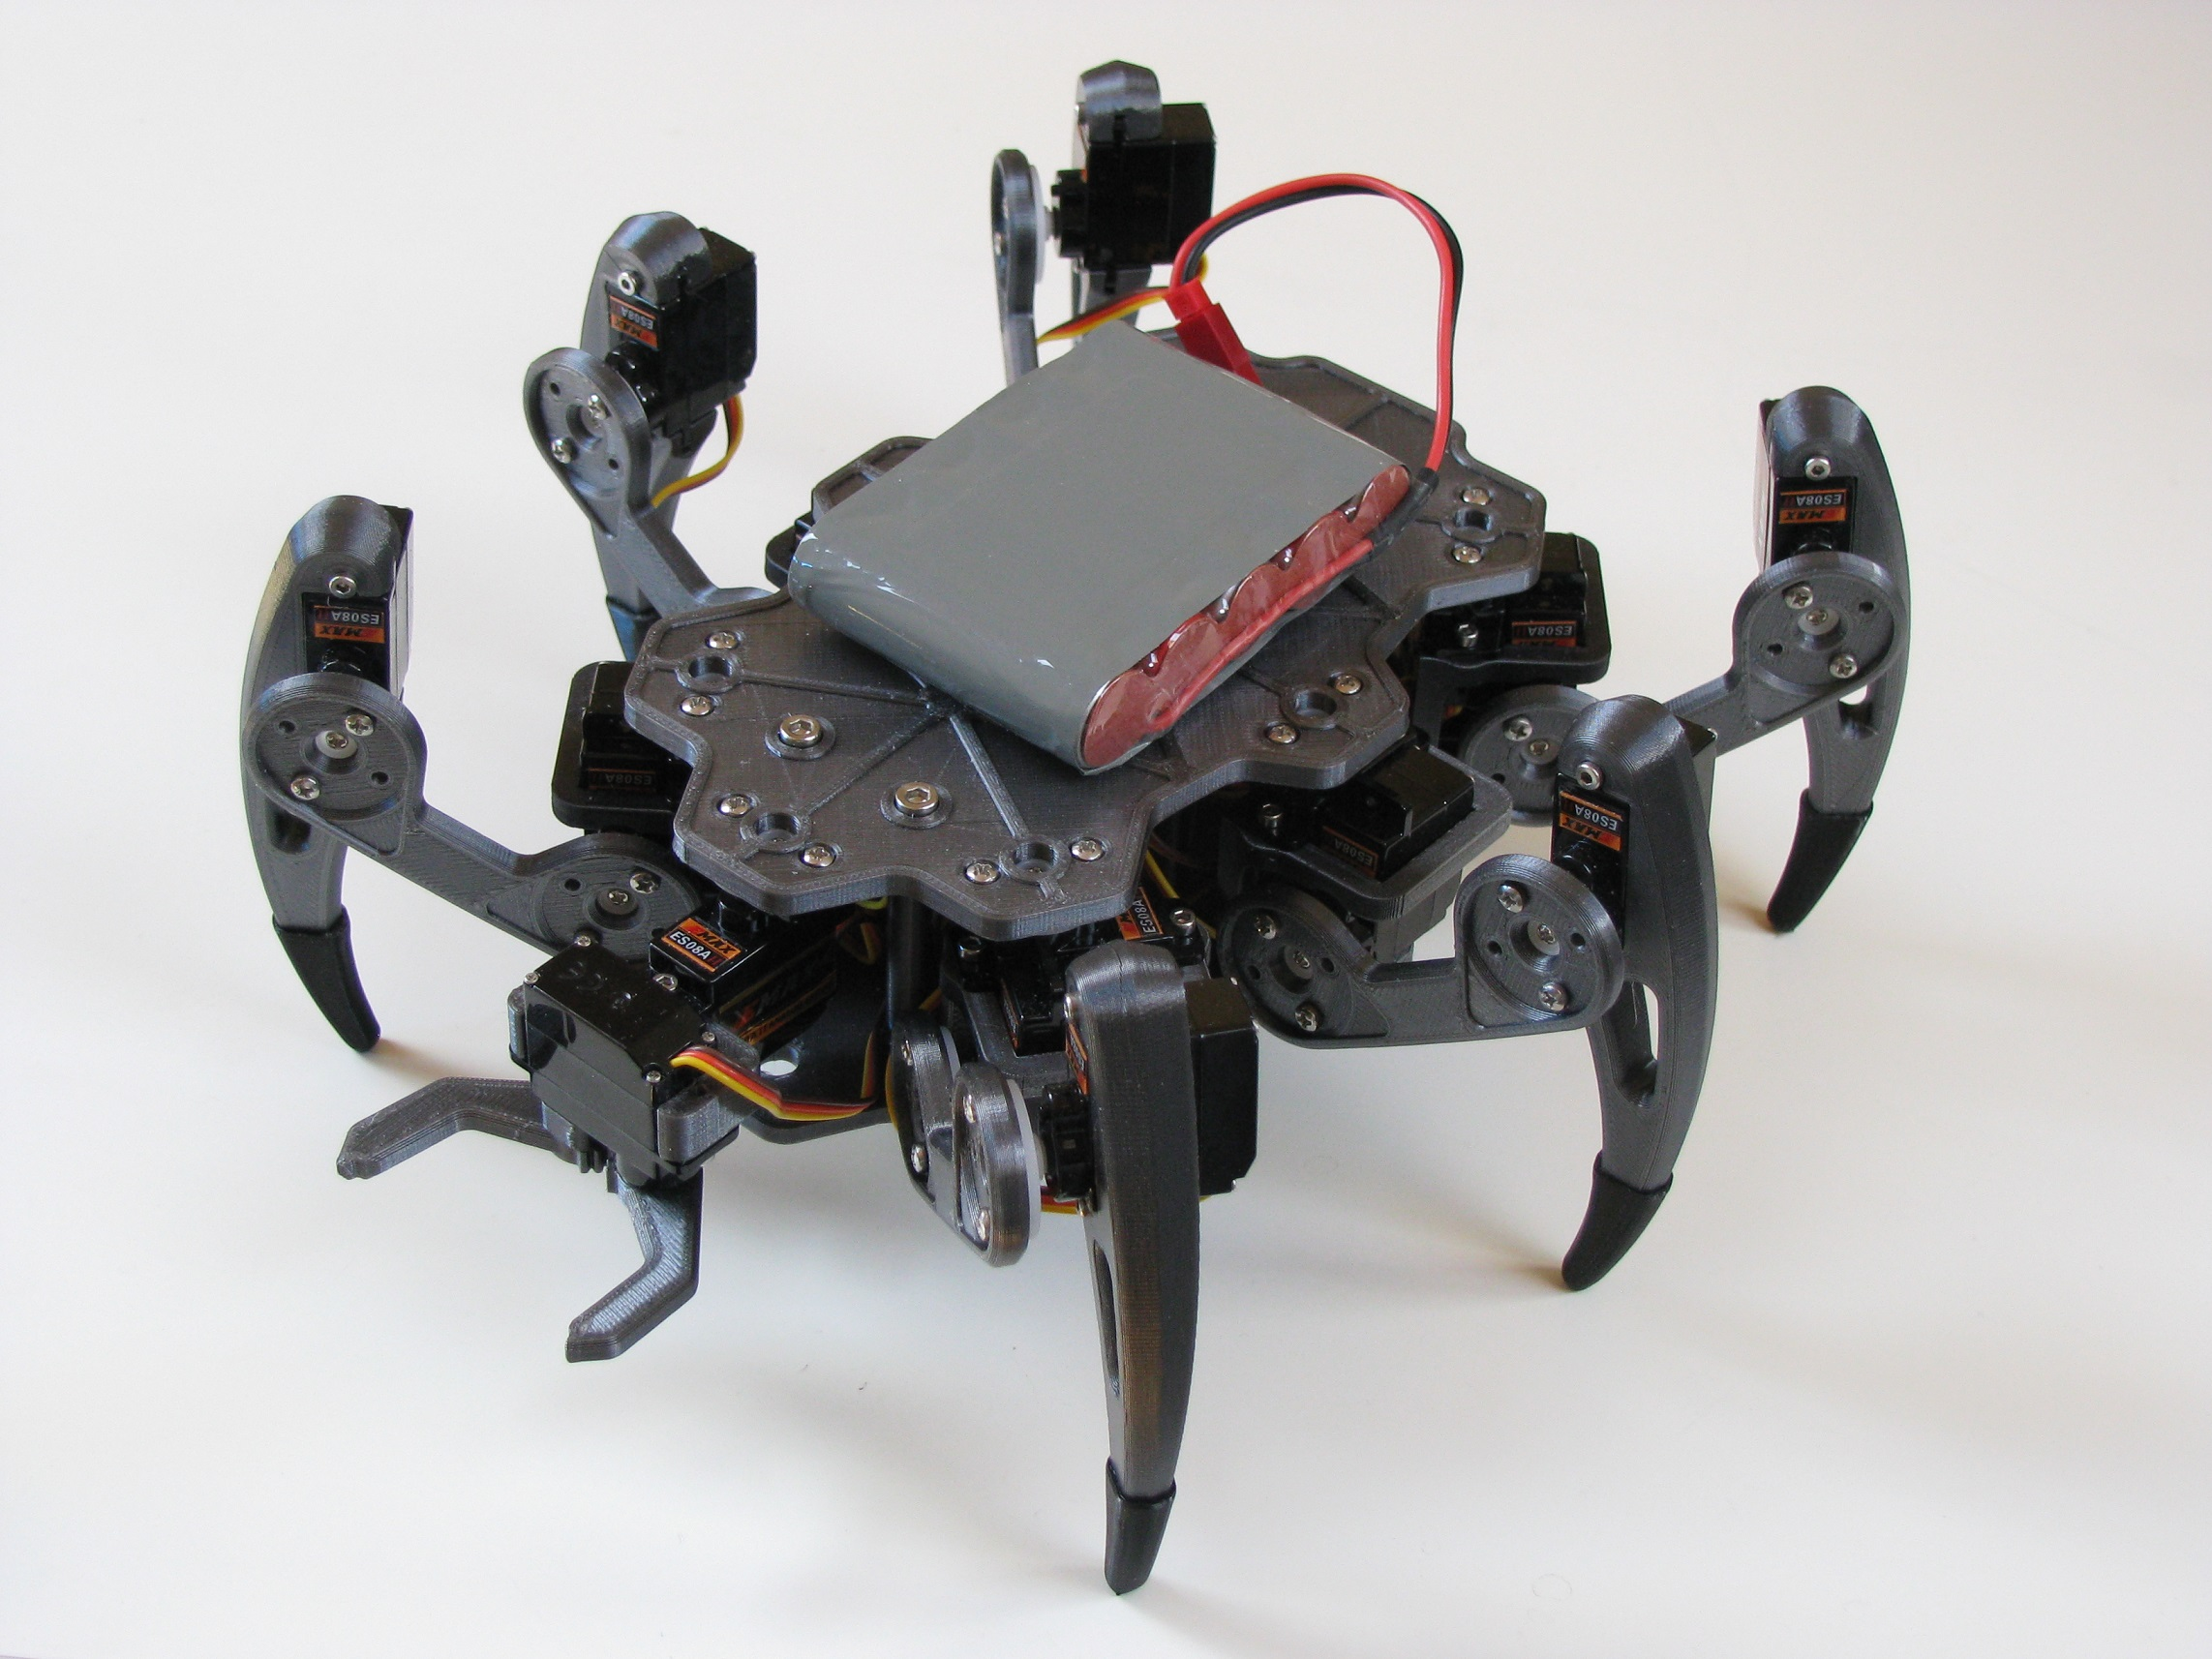
\includegraphics[width=0.43\textwidth]{img/zerobug.jpg}
    \caption[Proyecto ZeroBug]{ZeroBug\\[-2pt]{\footnotesize Fuente: Hackaday.io \cite{zerobug}.}}
    \label{fig:zerobug_wrap}
\end{wrapfigure}

También resultan relevantes algunos proyectos como ZeroBug \cite{zerobug} (ver Figura~\ref{fig:zerobug_wrap}) y los hexápodos de Hiwonder \cite{minihexa}, que exploran arquitecturas basadas en microcontroladores STM32/ESP32 y enfoques abiertos de desarrollo. En conjunto, estas iniciativas muestran cómo la frontera entre plataformas didácticas y sistemas de investigación se está reduciendo, permitiendo seleccionar una base mecánica accesible y complementarla con electrónica, software y capacidad de cómputo adaptadas a los objetivos del proyecto.


\section{Servomotores}
\label{sec:servomotores_inteligentes}

El control de los grados de libertad en plataformas robóticas requiere de servomotores que ofrezcan un equilibrio entre precisión, par mecánico y capacidad de integración. Los servomotores más populares son los controlados mediante una señal de modulación por ancho de pulsos (PWM), ya que son económicos y su implementación electrónica es sencilla.

\begin{wrapfigure}{r}{0.30\textwidth}
    \vspace{-25pt}
    \centering
    \captionsetup{justification=centering}
    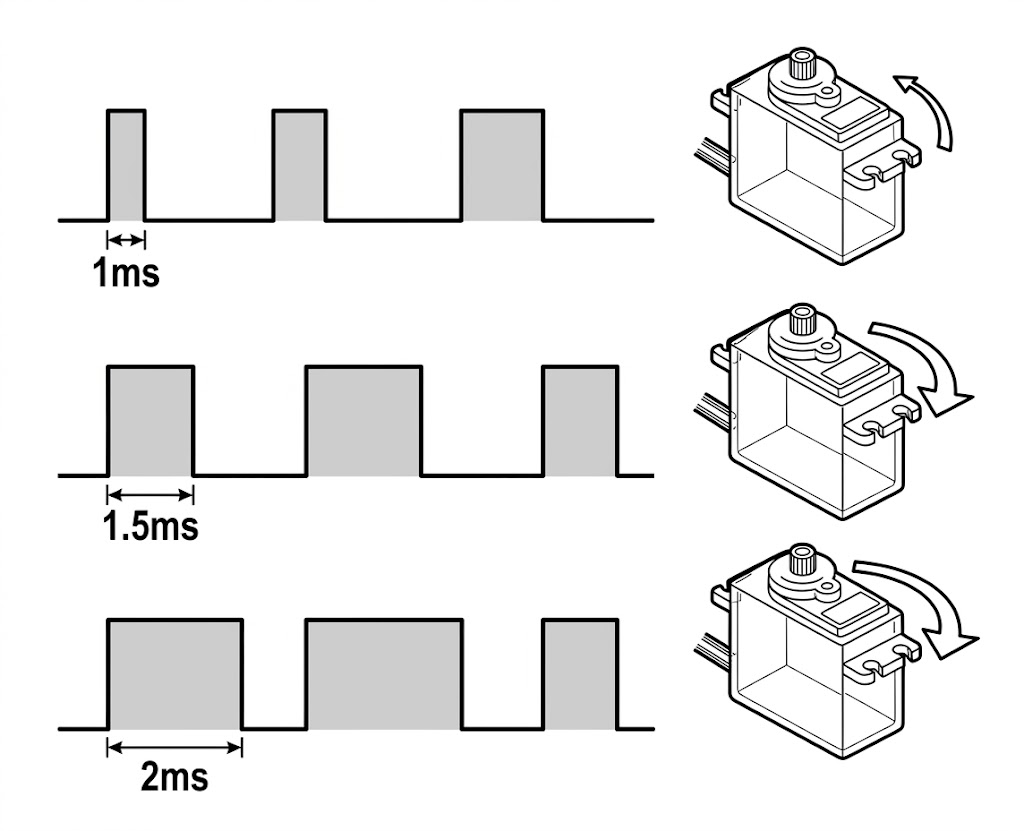
\includegraphics[width=0.30\textwidth]{img/servopwm.png}
    \caption[Control PWM de servomotores]{Control PWM de servomotores.\\{\footnotesize Fuente: Elaboración propia.}}
    \label{fig:pwm_control}
    \vspace{-20pt}
\end{wrapfigure}

Sin embargo, desde el punto de vista del controlador principal, estos presentan una limitación arquitectónica, ya que, aunque internamente disponen de un lazo cerrado de control de posición, dicha realimentación no sale del propio servomotor. El controlador se limita a enviar una onda cuadrada de alto nivel donde la duración del pulso fija la referencia angular, como se ilustra en la Figura~\ref{fig:pwm_control}, sin recibir a cambio ninguna información sensorial que confirme que el movimiento se haya realizado ni la posición real del eje. Esta ausencia de información sensorial hacia el controlador impide desarrollar un control de alto nivel o implementar rutinas de compensación dinámica que adapten la marcha del robot a las irregularidades del entorno. Para superar esta limitación, se recurre a los servomotores digitales. Estos dispositivos integran en un único encapsulado el motor de corriente continua, la electrónica de control, el sensor de posición y la interfaz de comunicación, como se muestra en la Figura~\ref{fig:ax12a_control}.

\begin{wrapfigure}{l}{0.35\textwidth}
    \vspace{-15pt}
    \centering
    \captionsetup{justification=centering}
    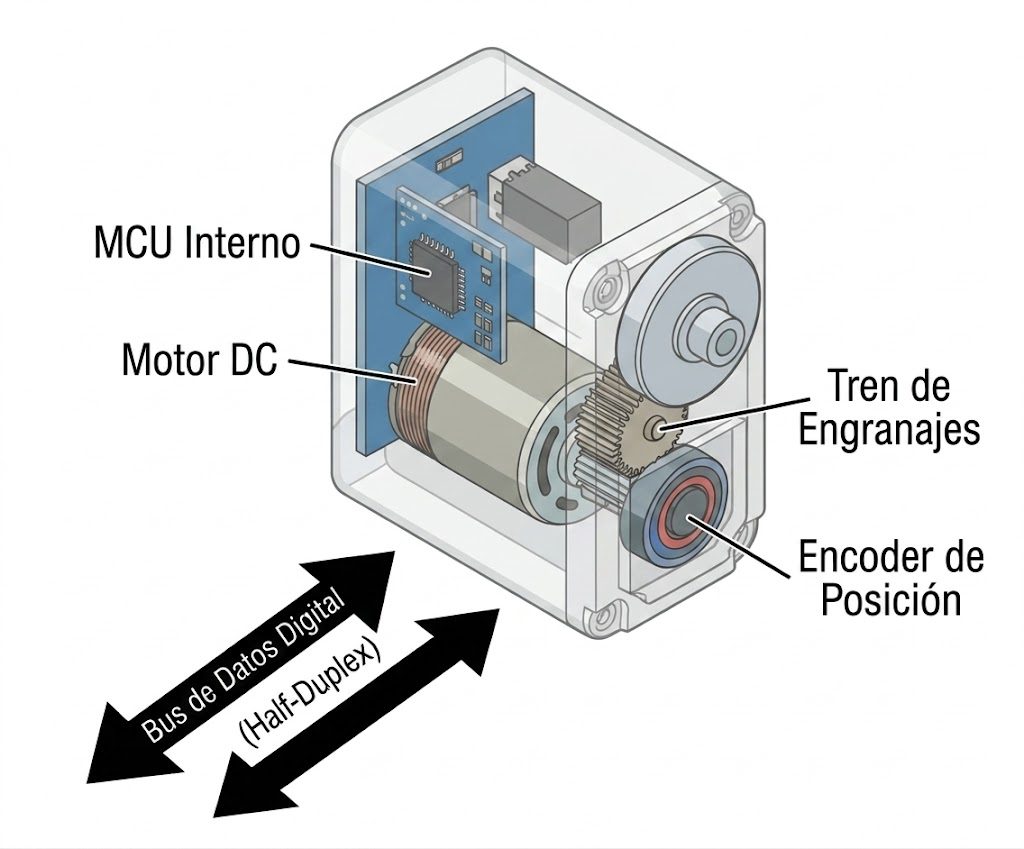
\includegraphics[width=0.35\textwidth]{img/servosmart.png}
    \caption[Arquitectura de servomotor digital]{Arquitectura de servomotor digital.\\{\footnotesize Fuente: Elaboración propia.}}
    \label{fig:ax12a_control}
    \vspace{-20pt}
\end{wrapfigure}

Esta arquitectura, basada en un control digital de posición/velocidad, les permite operar mediante paquetes de comunicación digital bidireccional, sustituyendo las señales analógicas unidireccionales por un protocolo serie asíncrono que, en muchos casos comerciales, se implementa en configuración \textit{half-duplex} \cite{ref_protocolo}. Además, se pueden consultar variables críticas como la posición del eje, la carga mecánica aplicada, la temperatura interna, el voltaje de alimentación y posibles alarmas de error. Otro aspecto relevante es la simplificación del cableado. El protocolo \textit{half-duplex} permite encadenar múltiples actuadores sobre una única línea de datos en topología \textit{daisy-chain}, tal y como se ilustra en la Figura~\ref{fig:half_duplex}.

\begin{wrapfigure}{r}{0.4\textwidth}
    \vspace{-6pt}
    \centering
    \captionsetup{justification=centering}
    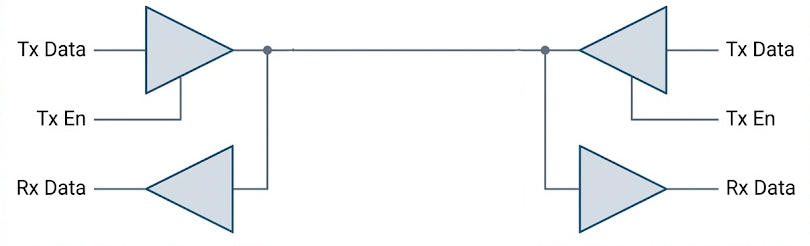
\includegraphics[width=0.4\textwidth]{img/half.png}
    \caption[Esquema de comunicación Half-Duplex]{Comunicación \textit{half-duplex}: transmisión bidireccional no simultánea sobre una única línea.\\{\footnotesize Fuente: Elaboración propia.}}
    \label{fig:half_duplex}
    \vspace{-20pt}
\end{wrapfigure}

Esto elimina la necesidad de cablear individualmente cada motor al controlador, reduciendo drásticamente la complejidad y el peso del cableado, un factor especialmente crítico en robots móviles donde cada gramo de masa no útil penaliza la autonomía y la dinámica del sistema.

En el contexto de este proyecto, se han seleccionado los actuadores DYNAMIXEL AX-12A \cite{ax12a_specs} como base motriz del hexápodo. Estos servomotores poseen todas las virtudes descritas y se comunican a través de un bus serie compartido que coordina de forma eficiente los 18~motores del sistema, tres por extremidad. Los detalles técnicos de sus capacidades mecánicas, protocolo de comunicación e integración hardware se abordan en profundidad en el Capítulo~\ref{cap:hardware}.

\section{ROS2 como arquitectura de integración robótica}

Robot Operating System (ROS) surgió como middleware de código abierto orientado a la robótica
\cite{quigley2009ros}. Se ha consolidado como estándar del sector por su modelo
de comunicación basado en publicadores y suscriptores, su ecosistema de paquetes
y su comunidad activa. ROS 1 presentaba
limitaciones estructurales que se hicieron más evidentes a medida que los casos
de uso evolucionaron. Destacaba su dependencia de un proceso centralizado llamado
\textit{rosmaster}, que actuaba como registro de nombres y punto de encuentro
entre nodos. Esta arquitectura introducía un punto único de fallo para el
descubrimiento y el registro. Si el proceso dejaba de estar disponible, las
conexiones ya establecidas podían mantenerse, pero no era posible registrar
nuevos nodos ni establecer nuevas conexiones. Además, utilizaba protocolos
de transporte TCPROS/UDPROS~\cite{ros_tcpros} que no soportan
de forma nativa la comunicación en tiempo real.

\begin{wrapfigure}{r}{0.5\textwidth}
    \vspace{-6pt}
    \centering
    \captionsetup{justification=centering}
    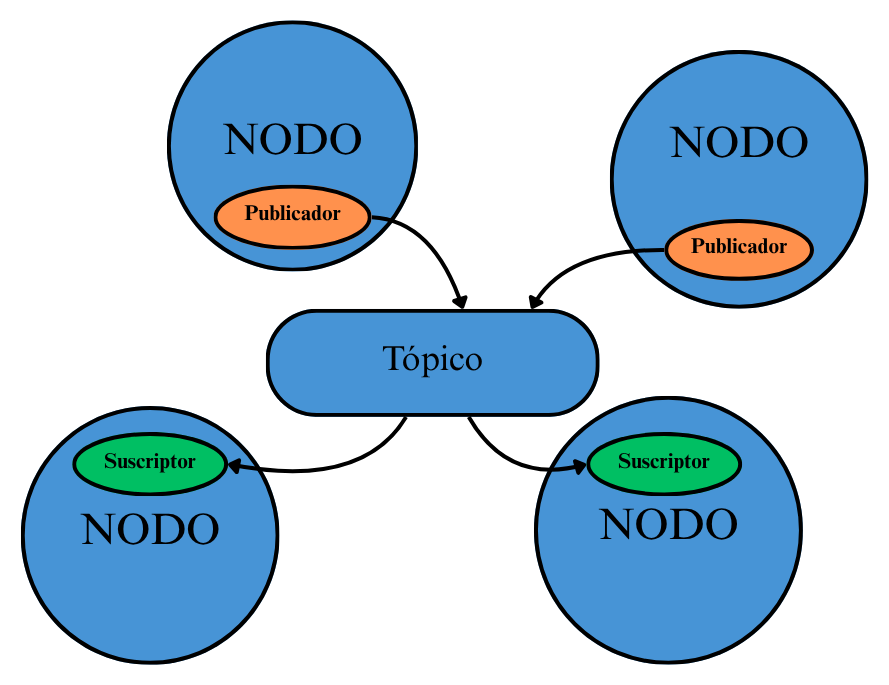
\includegraphics[width=0.5\textwidth]{img/ros2nodos.png}
    \caption[Modelo de comunicación de ROS]{Modelo de comunicación de ROS basado en nodos, tópicos, publicadores y suscriptores.\\{\footnotesize Fuente: Elaboración propia.}}
    \label{fig:ros_topics}
    \vspace{-10pt}
\end{wrapfigure}

Para resolver estas limitaciones, ROS~2 sustituyó TCPROS/UDPROS por DDS
(\textit{Data Distribution Service}), un estándar del Object Management Group
(OMG)~\cite{omg_dds}. ROS~2 elimina el \textit{rosmaster} mediante un protocolo
de descubrimiento descentralizado, de forma que cada nodo puede encontrar a los
demás sin depender de un proceso central. Sin embargo, ROS~2 presenta una limitación importante: ejecutarse sobre un
sistema operativo de propósito general como Linux no garantiza periodicidad
estricta en el bucle de control, ya que el planificador puede introducir
latencias no deterministas. Por ello, las arquitecturas habituales en robots
combinan ROS~2 con un microcontrolador que ejecuta un sistema en tiempo real.

El modelo de comunicación, basado en nodos, tópicos, publicadores y
suscriptores, se resume en la Figura~\ref{fig:ros_topics}. ROS~2 ofrece un ecosistema completo para robots móviles, con paquetes de navegación como Nav2~\cite{nav2}, que proporciona planificación de rutas,
evitación de obstáculos, localización y control de trayectorias, pudiendo
emplearse con distintas cinemáticas siempre que el robot se abstraiga como una
base móvil controlable. Para la percepción,
\texttt{slam\_toolbox}~\cite{slam_toolbox} permite
construir mapas en tiempo real mediante LiDAR, mientras que
\texttt{robot\_localization}~\cite{robot_localization} fusiona fuentes de
odometría e IMU. La visualización se realiza con RViz2~\cite{rviz2}, que
permite monitorizar el estado del robot, los tópicos activos y la nube de
puntos del sensor en tiempo real. Para la simulación, Gazebo~\cite{gazebo}
integra físicas, sensores virtuales y modelos, permitiendo validar algoritmos
antes de desplegarlos en hardware real. En conjunto, estas herramientas
convierten a ROS~2 en la plataforma para integrar un hexápodo como
nodo dentro de un sistema robótico completo, donde el control de bajo nivel
del microcontrolador se expone al resto del ecosistema.


\section{Trabajos previos en control de hexápodos}

El punto de partida natural para controlar el \textit{PhantomX} es el software
que la propia empresa Trossen Robotics distribuye para la plataforma: el \textit{PhantomX
Hexapod NUKE Sketch}, construido sobre NUKE (\textit{Nearly Universal Kinematics
Engine}) dentro del ecosistema ArbotiX/PyPose~\cite{nuke_hexapod}. Durante años ha
sido la forma más rápida de poner un \textit{PhantomX} a caminar sobre la placa
ArbotiX, y buena parte de su éxito como robot educativo se apoya en él. El
inconveniente es que su diseño ha envejecido: la cinemática del cuerpo se resuelve
con relaciones escalares en lugar de transformaciones homogéneas, la fase de vuelo
de la pata sigue un perfil triangular sin suavizado, y la generación de marcha, la
cinemática y la comunicación con los motores conviven en un mismo bloque
monolítico difícil de mantener o portar. Además, depende de la librería
BioloidController~\cite{bioloid_controller}, desarrollada por Vanadium Labs para la
ArbotiX, que no tiene port oficial en ESP-IDF~\cite{espidf}, el entorno de este proyecto.

Pero NUKE es solo una manera de resolver el problema, y el control de hexápodos se
ha abordado desde enfoques muy distintos. Uno de ellos es el bioinspirado, que no
parte de un modelo geométrico del robot, sino que deja que la marcha emerja de la
interacción entre osciladores y reflejos locales. Su versión más conocida son los
generadores centrales de patrones (\textit{Central Pattern Generators}, CPG)~\cite{ijspeert2008cpg},
redes de osciladores que imitan los circuitos neuronales de la locomoción animal y
producen marchas estables con muy pocos parámetros. El robot \textit{Genghis} del
MIT es el ejemplo clásico, con cada pata coordinándose con las demás sin un
planificador central~\cite{brooks1989robot}. Son enfoques robustos y adaptables,
aunque con ellos cuesta seguir trayectorias precisas o razonar sobre la postura
del cuerpo.

El enfoque contrario, y el más habitual cuando se busca precisión, es el control
basado en modelo. Aquí la posición de cada pata se calcula a partir de una
descripción cinemática rigurosa, normalmente con transformaciones homogéneas que
encadenan los sistemas de referencia del cuerpo, las caderas y los
eslabones~\cite{craig2018robotics}. Sobre esa base se planifican el apoyo, el vuelo
y la trayectoria del pie. Dentro de esta misma línea existen
controladores generalistas, pensados para reutilizarse en muchas plataformas. El
más representativo es OpenSHC~\cite{tam2020openshc}, integrado en ROS y con una
separación limpia entre cinemática, postura y marcha. Su punto débil es que se
apoya en cinemática inversa numérica y en una capacidad de cómputo que no encaja
con un microcontrolador sujeto a requisitos de tiempo real.

Ambas opciones presentan limitaciones evidentes para este proyecto: por un lado, NUKE
presenta una arquitectura muy acoplada y depende de una librería sin port oficial para
ESP-IDF, por otro, OpenSHC está orientado a equipos con mayor capacidad de cómputo y
emplea cinemática inversa numérica. Ninguno de los dos reunía al mismo tiempo la formulación geométrica, la
ejecución determinista en el ESP32 y la modularidad que se buscaban para el proyecto. En resumen, ante estas alternativas, en este TFG se optó por desarrollar un controlador propio
en lugar de adaptar uno existente.
